\subsection{Módulo de encendido/apagado de los procesadores}

Tras completar las actualizaciones del sistema operativo, el siguiente paso fue desarrollar una nueva funcionalidad enfocada en el control de los núcleos del procesador. Esta funcionalidad está diseñada para proporcionar una herramienta flexible que permita la gestión dinámica del encendido y apagado de los núcleos del procesador, con la expectativa de que futuros proyectos utilicen este módulo para optimizar el ahorro energético.

Este módulo es especialmente útil en escenarios donde la carga de trabajo varía significativamente, permitiendo controlar los núcleos durante periodos de baja demanda y ajustarlos cuando la carga aumenta. Aunque aún no se ha implementado una estrategia de ahorro energético, esta herramienta abre la puerta a desarrollos futuros que podrían aprovechar esta capacidad para reducir el consumo de energía y mejorar la eficiencia del sistema.

\subsubsection{Objetivos}

El objetivo general de esta sección, fue el desarrollo de una nueva funcionalidad dentro del \textit{scheduler} del sistema operativo FreeBSD que permita habilitar o deshabilitar los diferentes núcleos del procesador de manera dinámica y eficiente.

Este objetivo principal se traduce en múltiples aplicaciones que pueden proporcionar ventajas significativas, tales como la optimización del uso de recursos de hardware bajo cargas de trabajo reducidas, la restricción de núcleos disponibles para aplicaciones específicas, y la capacidad de ajustar el estado de los procesadores en tiempo de ejecución. Estas aplicaciones subrayan la importancia de una solución flexible, que permita la adaptación dinámica del manejo de núcleos en diversas partes del sistema, respondiendo eficazmente a una variedad de situaciones operativas.

\subsubsection{Primera Iteración: Implementación del Módulo de Encendido/Apagado mediante cambios en la Red de Petri}

Para iniciar la implementación del módulo de encendido/apagado de núcleos del procesador, se debatieron dos enfoques relacionados con la Red de Petri del sistema operativo. El primer enfoque proponía utilizar las plazas y transiciones ya existentes, estableciendo diferentes políticas a través de cambios en el código del \textit{scheduler}. El segundo enfoque, que fue el adoptado finalmente, implicaba la incorporación de nuevas plazas y transiciones en la Red de Petri para representar explícitamente el estado de los núcleos del procesador. Optamos por esta segunda opción porque nos permitió integrar el módulo de manera más fluida al sistema ya existente, sin hacer cambios drásticos en el núcleo del sistema operativo, y ampliando al mismo tiempo las capacidades de la Red de Petri. La principal ventaja de esta implementación, y motivador principal, fue que desde cualquier parte del sistema, simplemente disparando una transición, fuera posible activar o desactivar cualquier núcleo del procesador según sea necesario.

Con esta decisión en mente, el primer paso fue crear un indicador que permitiera conocer si cada procesador está encendido o apagado. Para esto, se añadió una nueva plaza en la Red de Petri, llamada \texttt{PLACE\_SUSPENDED}. La presencia o ausencia de un \textit{token} en esta plaza indica si un procesador está disponible para encolar y ejecutar hilos.

La plaza \texttt{PLACE\_SUSPENDED} está acompañada de dos transiciones que manejan el \textit{token} correspondiente: \texttt{TRAN\_SUSPEND\_PROC} para deshabilitar el núcleo, y \texttt{TRAN\_WAKEUP\_PROC} para habilitarlo nuevamente. Se añadió un arco inhibidor a la transición que libera el recurso para asegurar que la plaza funcione como un recurso único. Una vez que un procesador está deshabilitado, solo la transición que lo habilita de nuevo queda sensibilizada.

En resumen, la plaza \texttt{PLACE\_SUSPENDED} controla las transiciones de encolado tanto de la cola específica del CPU como de la cola global. Cuando el CPU está suspendido, impide que nuevos hilos se añadan a su cola y se ejecuten. Sin embargo, es importante destacar que este desarrollo no elimina los hilos que ya estaban en la cola del CPU antes de que se deshabilitara. Es decir, los hilos ya encolados seguirán siendo ejecutados, pero no podrán volver a la cola del CPU inhabilitado. Esta lógica está reflejada en la Red de Petri, donde la nueva plaza de suspensión solo afecta a las transiciones de encolado y desencolado, sin interferir en la ejecución de hilos ni en la transición específica de desencolado del procesador (\texttt{TRAN\_UNQUEUE}).

\begin{figure}[H]
    \centering
    \vspace*{0.1in}
    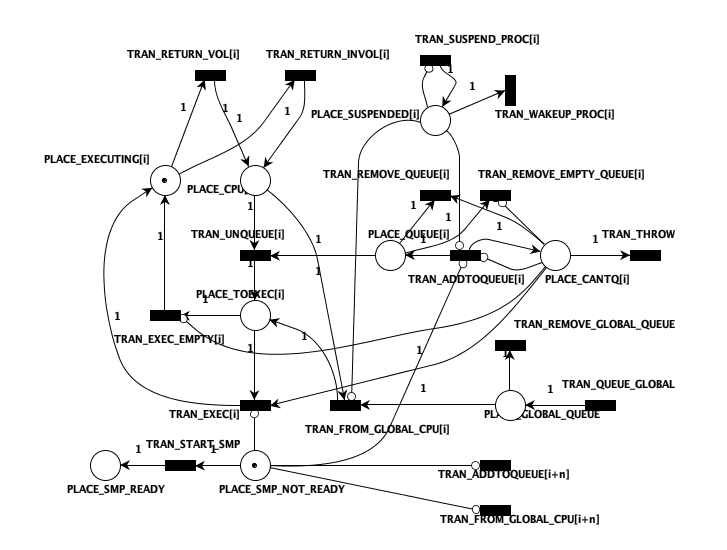
\includegraphics[width=0.8\textwidth]{./images/cpuOnOff-1st-iteration.png}
    \caption{Primera iteración del módulo de encendido/apagado de núcleos del procesador.}
    \label{fig:queueing-structure}
\end{figure}

Como primer paso para implementar esta funcionalidad a nivel de código, nos centramos en ajustar las matrices fundamentales que soportan el funcionamiento de la Red de Petri: la matriz base y la matriz de incidencia. Estas matrices son cruciales para la representación y el manejo de las transiciones y plazas en la Red de Petri.\par

La matriz base, que define la estructura inicial de la Red de Petri, necesitaba ser actualizada para reflejar las nuevas plazas y transiciones introducidas. Específicamente, agregamos entradas para la nueva plaza \texttt{PLACE\_SUSPENDED} y las transiciones asociadas (\texttt{TRAN\_SUSPEND\_PROC} y \texttt{TRAN\_WAKEUP\_PROC}). Esta modificación asegura que la estructura de la red pueda manejar los cambios en el estado de los núcleos del procesador, permitiendo que el sistema registre y gestione correctamente los \textit{tokens} en la plaza de suspensión.\par

\renewcommand{\arraystretch}{1.5}
\setlength{\tabcolsep}{10pt}

\begin{table}[H]
    \centering
    \begin{tabular}{|c|c|c|c|c|c|c|c|c|}
        \hline
        1 & 0 & -1 & 0 & 0 & 0 & 0 & -1 & 0 \\
        \hline
        1 & -1 & 0 & 0 & 0 & 0 & 0 & -1 & -1 \\
        \hline
        0 & -1 & 0 & 0 & 1 & 1 & -1 & 0 & 0 \\
        \hline
        0 & 1 & -1 & -1 & 0 & 0 & 1 & 0 & 0 \\
        \hline
        0 & 0 & 1 & 1 & -1 & -1 & 0 & 0 & 0 \\
        \hline
    \end{tabular}
    \caption{Matriz base inicial.}
    \label{tabla:matriz_base_pre}
\end{table}

\begin{table}[H]
    \centering
    \begin{tabular}{|c|c|c|c|c|c|c|c|c|c|c|}
        \hline
        1 & 0 & -1 & 0 & 0 & 0 & 0 & -1 & 0 & \cellcolor{lightgray}0 & \cellcolor{lightgray}0 \\
        \hline
        1 & -1 & 0 & 0 & 0 & 0 & 0 & -1 & -1 & \cellcolor{lightgray}0 & \cellcolor{lightgray}0 \\
        \hline
        0 & -1 & 0 & 0 & 1 & 1 & -1 & 0 & 0 & \cellcolor{lightgray}0 & \cellcolor{lightgray}0 \\
        \hline
        0 & 1 & -1 & -1 & 0 & 0 & 1 & 0 & 0 & \cellcolor{lightgray}0 & \cellcolor{lightgray}0 \\
        \hline
        0 & 0 & 1 & 1 & -1 & -1 & 0 & 0 & 0 & \cellcolor{lightgray}0 & \cellcolor{lightgray}0 \\
        \hline
        \cellcolor{lightgray}0 & \cellcolor{lightgray}0 & \cellcolor{lightgray}0 & \cellcolor{lightgray}0 & \cellcolor{lightgray}0 & \cellcolor{lightgray}0 & \cellcolor{lightgray}0 & \cellcolor{lightgray}0 & \cellcolor{lightgray}0 & \cellcolor{lightgray}1 & \cellcolor{lightgray}-1 \\
        \hline
    \end{tabular}
    \caption{Matriz base: Primera iteración del módulo de encendido/apagado.}
    \label{tabla:matriz_base_post}
\end{table}

Por otro lado, la matriz de incidencia describe cómo las transiciones afectan a las plazas y viceversa. Actualizar esta matriz implicó modificar las relaciones entre las nuevas transiciones y las plazas afectadas. Concretamente, tuvimos que ajustar las entradas para reflejar el impacto de las transiciones de habilitación y deshabilitación de los núcleos en las plazas correspondientes. Esto incluye la configuración de los arcos inhibidores que garantizan que los cambios en el estado del procesador se gestionen correctamente.\par

\renewcommand{\arraystretch}{1.5}
\setlength{\tabcolsep}{10pt}

\begin{table}[H]
    \centering
    \begin{tabular}{|c|c|c|c|c|c|c|c|c|}
        \hline
        1 & 0 & 0 & 1 & 0 & 0 & 0 & 0 & 1 \\
        \hline
        0 & 0 & 0 & 0 & 0 & 0 & 0 & 0 & 0 \\
        \hline
        0 & 0 & 0 & 0 & 0 & 0 & 0 & 0 & 0 \\
        \hline
        0 & 0 & 0 & 0 & 0 & 0 & 0 & 0 & 0 \\
        \hline
        0 & 0 & 0 & 0 & 0 & 0 & 0 & 0 & 0 \\
        \hline
    \end{tabular}
    \caption{Matriz de incidencia inicial.}
    \label{tabla:matriz_incidencia_pre}
\end{table}

\begin{table}[H]
    \centering
    \begin{tabular}{|c|c|c|c|c|c|c|c|c|c|c|}
        \hline
        1 & 0 & 0 & 1 & 0 & 0 & 0 & 0 & 1 & \cellcolor{lightgray}0 & \cellcolor{lightgray}0 \\
        \hline
        0 & 0 & 0 & 0 & 0 & 0 & 0 & 0 & 0 & \cellcolor{lightgray}0 & \cellcolor{lightgray}0 \\
        \hline
        0 & 0 & 0 & 0 & 0 & 0 & 0 & 0 & 0 & \cellcolor{lightgray}0 & \cellcolor{lightgray}0 \\
        \hline
        0 & 0 & 0 & 0 & 0 & 0 & 0 & 0 & 0 & \cellcolor{lightgray}0 & \cellcolor{lightgray}0 \\
        \hline
        0 & 0 & 0 & 0 & 0 & 0 & 0 & 0 & 0 & \cellcolor{lightgray}0 & \cellcolor{lightgray}0 \\
        \hline
        \cellcolor{lightgray}1 & \cellcolor{lightgray}0 & \cellcolor{lightgray}0 & \cellcolor{lightgray}0 & \cellcolor{lightgray}0 & \cellcolor{lightgray}0 & \cellcolor{lightgray}1 & \cellcolor{lightgray}0 & \cellcolor{lightgray}0 & \cellcolor{lightgray}1 & \cellcolor{lightgray}0 \\
        \hline
    \end{tabular}
    \caption{Matriz de incidencia: Primera iteración del módulo de encendido/apagado.}
    \label{tabla:matriz_incidencia_post}
\end{table}

Como parte de los ajustes realizados en las matrices, se incorporó una nueva función, \textit{toggle\_active\_cpu}, al archivo de métodos auxiliares de la Red de Petri. Esta función puede ser invocada desde un módulo del kernel y está diseñada para alternar el estado de un CPU especificado como parámetro. La función verifica si la transición asociada está sensibilizada y, si es así, procede a dispararla. En resumen, esta adición permite seleccionar y alternar el estado de un procesador, que puede ser suspendido o activado según sea necesario, y se gestiona de manera externa al flujo principal del kernel, permitiendo así un control en tiempo real del estado de habilitación del CPU.\par

Tras la implementación de esta funcionalidad, nos encontramos con un problema inesperado: la funcionalidad no se comportaba como se había previsto. Específicamente, recibimos alertas indicando que algunas transiciones no estaban sensibilizadas durante los intentos de disparo. EL proceso de depuración reveló que el problema estaba relacionado con el comportamiento del \textit{scheduler} cuando no había hilos disponibles para ejecutar, ni en la cola local del procesador ni en la cola global.

En la siguiente sección, se describe la solución implementada para superar esta dificultad.

\subsubsection{Segunda Iteración: Soporte del \textit{idlethread} en la Red de Petri}

Durante la depuración realizada en la iteración anterior, se identificó un error en situaciones donde una CPU no tenía hilos listos para ejecutar. Para abordar este problema en la segunda iteración del módulo de encendido/apagado, es crucial entender el papel del \textit{idlethread}. En estos casos, el scheduler encola y ejecuta el \textit{idlethread}, una funcionalidad que ya estaba presente antes del inicio del proyecto integrador y que es característica del scheduler 4.4BSD utilizado en FreeBSD.\par

El \textit{idlethread} es un hilo \textit{dummy}, es decir, un hilo que no genera carga significativa para el procesador. Puede ser encolado, suspendido y ejecutado de manera similar a otros hilos. Cada núcleo de CPU tiene asociado su propio \textit{idlethread}, el cual ejecuta un bucle simple que generalmente consiste en poner la CPU en un estado de bajo consumo o realizar otras operaciones de ahorro energético. De esta manera, el \textit{idlethread} asegura que la CPU permanezca ocupada incluso cuando no hay tareas o hilos listos para ejecutarse. En lugar de dejar que un núcleo de CPU esté inactivo, FreeBSD utiliza el \textit{idlethread} para mantener el procesador ocupado, equilibrando así el consumo de energía y el rendimiento general del sistema.\par

Cuando no hay hilos o procesos ejecutables listos para ejecutarse en una CPU, el scheduler selecciona el \textit{idlethread} como el siguiente hilo a ejecutar. Dado que el \textit{idlethread} tiene la prioridad más baja, solo se programa cuando no hay tareas de mayor prioridad disponibles. En cualquier momento en que aparezca un hilo de mayor prioridad, el \textit{idlethread} será reemplazado por este nuevo hilo que requiere tiempo de procesador.\par

Nuestra Red de Petri no contemplaba el caso específico del \textit{idlethread}. Como resultado, en ausencia de hilos a planificar, se intentaban disparar transiciones \texttt{TRAN\_UNQUEUE} para los planificadores correspondientes, lo que provocaba fallas en el sistema de la red y desajustes en las plazas asociadas.\par

Para resolver esta problemática, decidimos añadir una nueva transición, \texttt{TRAN\_EXEC\_IDLE}, que permite la ejecución del \textit{idlethread} cuando no hay hilos en la cola del procesador, incluyendo el caso en que el CPU está suspendido. Tras implementar estos cambios, el modelo comenzó a representar con precisión el proceso interno del planificador.\par

\begin{figure}[H]
    \centering
    \vspace*{0.1in}
    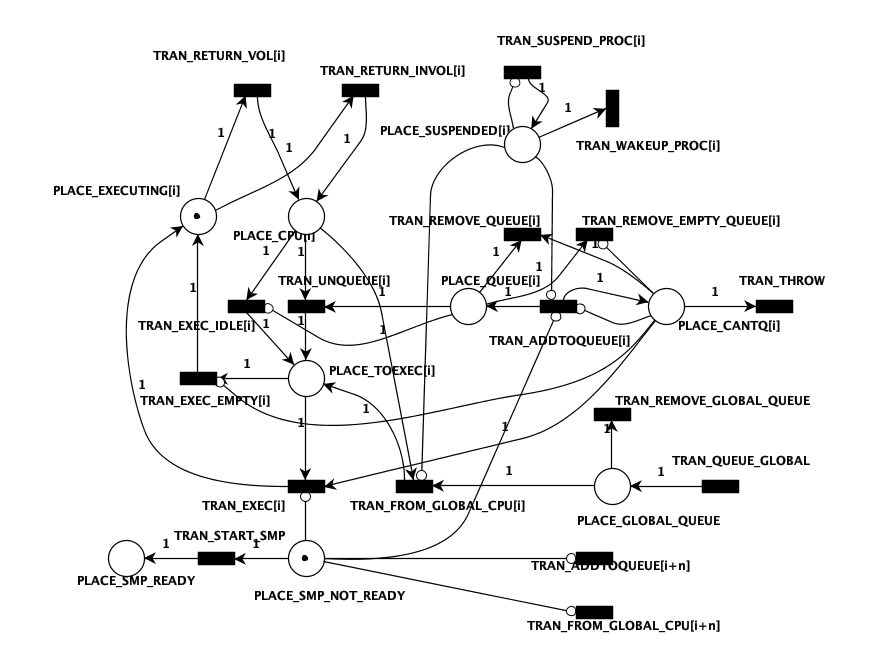
\includegraphics[width=0.8\textwidth]{./images/cpuOnOff-2nd-iteration.png}
    \caption{Segunda iteración del módulo de encendido/apagado de núcleos del procesador.}
    \label{fig:queueing-structure}
\end{figure}

Una vez más, la implementación de estos cambios, comenzó por el cambio de las matrices base y de incidencia.

\begin{table}[H]
    \centering
    \begin{tabular}{|c|c|c|c|c|c|c|c|c|c|c|c|}
        \hline
        1 &  0 & -1 &  0 & \cellcolor{lightgray}0 & 0 & 0 & 0 & -1 & 0 & 0 & 0 \\
        \hline
        1 & -1 &  0 &  0 & \cellcolor{lightgray}0 & 0 & 0 & 0 & -1 & -1 & 0 & 0 \\
        \hline
        0 & -1 &  0 &  0 & \cellcolor{lightgray}-1 & 1 & 1 & -1 & 0 & 0 & 0 & 0 \\
        \hline
        0 &  1 & -1 & -1 & \cellcolor{lightgray}1 & 0 & 0 & 1 & 0 & 0 & 0 & 0 \\
        \hline
        0 &  0 &  1 &  1 & \cellcolor{lightgray}0 & -1 & -1 & 0 & 0 & 0 & 0 & 0 \\
        \hline
        0 &  0 &  0 &  0 & \cellcolor{lightgray}0 & 0 & 0 & 0 & 0 & 0 & 1 & -1 \\
        \hline
    \end{tabular}
    \caption{Matriz base: Segunda iteración del módulo de encendido/apagado.}
    \label{tabla:matriz_base_post_2}
\end{table}

\begin{table}[H]
    \centering
    \begin{tabular}{|c|c|c|c|c|c|c|c|c|c|c|c|}
        \hline
        1 & 0 & 0 & 1 & \cellcolor{lightgray}0 & 0 & 0 & 0 & 0 & 1 & 0 & 0 \\
        \hline
        0 & 0 & 0 & 0 & \cellcolor{lightgray}1 & 0 & 0 & 0 & 0 & 0 & 0 & 0 \\
        \hline
        0 & 0 & 0 & 0 & \cellcolor{lightgray}0 & 0 & 0 & 0 & 0 & 0 & 0 & 0 \\
        \hline
        0 & 0 & 0 & 0 & \cellcolor{lightgray}0 & 0 & 0 & 0 & 0 & 0 & 0 & 0 \\
        \hline
        0 & 0 & 0 & 0 & \cellcolor{lightgray}0 & 0 & 0 & 0 & 0 & 0 & 0 & 0 \\
        \hline
        1 & 0 & 0 & 0 & \cellcolor{lightgray}0 & 0 & 0 & 1 & 0 & 0 & 1 & 0 \\
        \hline
    \end{tabular}
    \caption{Matriz de incidencia: Segunda iteración del módulo de encendido/apagado.}
    \label{tabla:matriz_incidencia_post_2}
\end{table}


%% TODO ACA ME QUEDE: Esto de abajo hay que revisarlo

Además de modificar el archivo base de la Red de Petri, se agregaron cambios dentro de la función sched\_choose (encargada de indicar cuál es el mejor hilo a ejecutar) del planificador para que en los casos de CPU suspendido, el hilo elegido para pasar a ejecución sea el idlethread hasta que el procesador se activado nuevamente.\par

Para lograr esto, se consulta directamente a través de una función, si la plaza de suspensión del procesador que se encuentra ejecutando el código, contiene algún token. En caso de que esto sea verdadero, estaríamos ante la presencia de un procesador suspendido. Caso contrario el funcionamiento es el habitual.\par


\subsubsection{Resultados}

Una vez finalizado el desarrollo de esta nueva funcionalidad pudimos comenzar a realizar las pruebas pertinentes.\par

En resúmen, la funcionalidad propuesta para el planificador, que permite habilitar o inhabilitar núcleos del procesador, ha sido resuelta permitiendo así un control sobre los mismos que previamente no existía.\par

A su vez, se logró la versatilidad propuesta para este módulo, ya que es posible poner en funcionamiento esta mejora en tiempo real sin necesidad de reiniciar el sistema operativo.\par

Los detalles de los resultados serán explicados con mayor profundidad en el capítulo de
“Análisis de resultados”.\par

Un detalle a tener en cuenta es la imposibilidad de suspender el procesador cero. Esto es debido a que el sistema operativo utiliza este núcleo por defecto para tareas esenciales y al apagarlo, el sistema comienza a ralentizarse hasta que el kernel entra en pánico, resultando en un reinicio del mismo.\par

Para evitar que esta situación pueda darse, se realizaron los cambios necesarios en el código para prohibir la elección del núcleo en cuestión.\par


\subsubsection{Próximos pasos}

La implementación de este módulo no tiene mejoras o impacto inmediato en el sistema;  debido a que es un módulo independiente, activado mediante una señal enviada en un momento elegido por el desarrollador.\par

Observando a futuro, creemos que el próximo enfoque debería apuntar a una integración de esta funcionalidad con elementos propios del sistema operativo, tales como hilos, procesos o programas que controlen los mismos.\par

De esta forma se cambiaría el estado de los procesadores en tiempo real y de acuerdo a necesidades reales del sistema en conjunto; no solo a través de un módulo de kernel.\par
